\documentclass[tikz]{standalone}% 'crop' is the default for v1.0, before it was 'preview'
\usetikzlibrary{positioning,matrix,shapes,arrows,calc,fit}

\pgfdeclareimage[height=1cm]{ngreen}{img/ngreen.pdf}
\pgfdeclareimage[height=1cm]{nblue}{img/nblue.pdf}
\pgfdeclareimage[height=1cm]{nred}{img/nred.pdf}
\pgfdeclareimage[height=1cm]{nblack}{img/nblack.pdf}

%\usetikzlibrary{...}% tikz package already loaded by 'tikz' option
\begin{document}
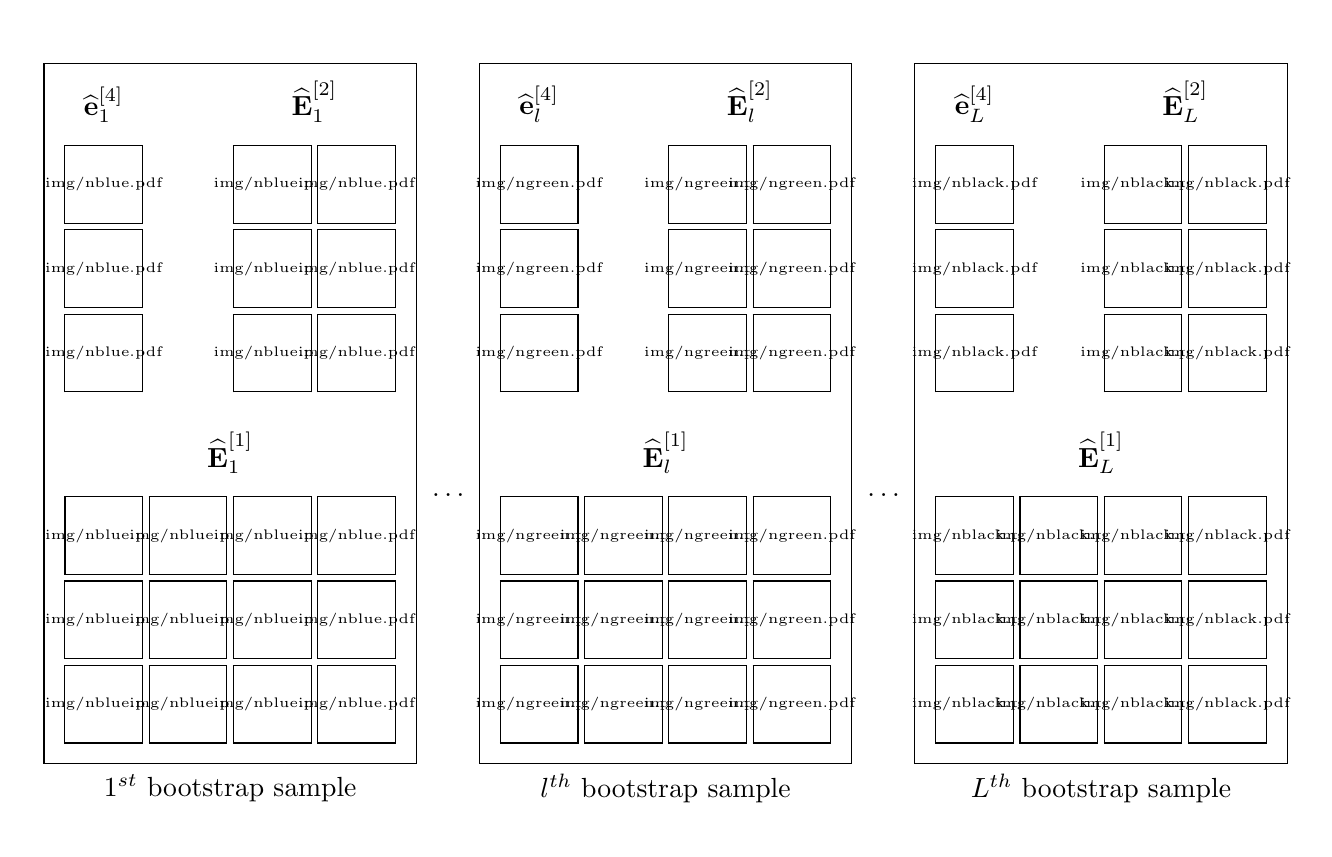
\begin{tikzpicture}
\matrix (e1) [matrix of nodes,row sep=0cm,column sep=0cm, nodes= {rectangle, fill=white, inner sep = 1pt}, label={[name=labe1] above:{$\widehat{\textbf{E}}_1^{[1]}$}}]
{
\pgfuseimage{nblue} & \pgfuseimage{nblue} & \pgfuseimage{nblue} & \pgfuseimage{nblue}\\
\pgfuseimage{nblue} & \pgfuseimage{nblue} & \pgfuseimage{nblue} & \pgfuseimage{nblue}\\
\pgfuseimage{nblue} & \pgfuseimage{nblue} & \pgfuseimage{nblue} & \pgfuseimage{nblue}\\
};

\matrix (ek) [above= 10mm of e1.north east,
       anchor=south east, matrix of nodes,row sep=0cm,column sep=0cm, nodes= {rectangle, fill=white, inner sep = 1pt}, label={[name=labek] above:{$\widehat{\textbf{E}}_1^{[2]}$}}]
{
\pgfuseimage{nblue} & \pgfuseimage{nblue} \\
\pgfuseimage{nblue} & \pgfuseimage{nblue} \\
\pgfuseimage{nblue} & \pgfuseimage{nblue} \\
};

\matrix (em) [above= 10mm of e1.north west,
       anchor=south west, matrix of nodes,row sep=0cm,column sep=0cm, nodes= {rectangle, fill=white, inner sep = 1pt}, label={[name=labem] above:{$\widehat{\textbf{e}}_1^{[4]}$}}]
{
\pgfuseimage{nblue} \\
\pgfuseimage{nblue} \\
\pgfuseimage{nblue} \\
};


\node[right= 1.75mm of e1.north east,
       anchor=north west] {$\dots$};
\matrix (e1_l) [right= 10mm of e1.north east,
       anchor=north west, matrix of nodes,row sep=0cm,column sep=0cm, nodes= {rectangle, fill=white, inner sep = 1pt}, label={[name=labe1l] above:{$\widehat{\textbf{E}}_l^{[1]}$}}]
{
\pgfuseimage{ngreen} & \pgfuseimage{ngreen} & \pgfuseimage{ngreen} & \pgfuseimage{ngreen}\\
\pgfuseimage{ngreen} & \pgfuseimage{ngreen} & \pgfuseimage{ngreen} & \pgfuseimage{ngreen}\\
\pgfuseimage{ngreen} & \pgfuseimage{ngreen} & \pgfuseimage{ngreen} & \pgfuseimage{ngreen}\\
};

\matrix (ek_l) [above= 10mm of e1_l.north east,
       anchor=south east, matrix of nodes,row sep=0cm,column sep=0cm, nodes= {rectangle, fill=white, inner sep = 1pt}, label={[name=labekl] above:{$\widehat{\textbf{E}}_l^{[2]}$}}]
{
\pgfuseimage{ngreen} & \pgfuseimage{ngreen} \\
\pgfuseimage{ngreen} & \pgfuseimage{ngreen} \\
\pgfuseimage{ngreen} & \pgfuseimage{ngreen} \\
};

\matrix (em_l) [above= 10mm of e1_l.north west,
       anchor=south west, matrix of nodes,row sep=0cm,column sep=0cm, nodes= {rectangle, fill=white, inner sep = 1pt}, label={[name=labeml] above:{$\widehat{\textbf{e}}_l^{[4]}$}}]
{
\pgfuseimage{ngreen} \\
\pgfuseimage{ngreen} \\
\pgfuseimage{ngreen} \\
};

\node[right= 1.75mm of e1_l.north east,
       anchor=north west] {$\dots$};
\matrix (e1_L) [right= 10mm of e1_l.north east,
       anchor=north west, matrix of nodes,row sep=0cm,column sep=0cm, nodes= {rectangle, fill=white, inner sep = 1pt}, label={[name=labe1L] above:{$\widehat{\textbf{E}}_L^{[1]}$}}]
{
\pgfuseimage{nblack} & \pgfuseimage{nblack} & \pgfuseimage{nblack} & \pgfuseimage{nblack}\\
\pgfuseimage{nblack} & \pgfuseimage{nblack} & \pgfuseimage{nblack} & \pgfuseimage{nblack}\\
\pgfuseimage{nblack} & \pgfuseimage{nblack} & \pgfuseimage{nblack} & \pgfuseimage{nblack}\\
};


\matrix (ek_L) [above= 10mm of e1_L.north east,
       anchor=south east, matrix of nodes,row sep=0cm,column sep=0cm, nodes= {rectangle, fill=white, inner sep = 1pt}, label={[name=labekL] above:{$\widehat{\textbf{E}}_L^{[2]}$}}]
{
\pgfuseimage{nblack} & \pgfuseimage{nblack} \\
\pgfuseimage{nblack} & \pgfuseimage{nblack} \\
\pgfuseimage{nblack} & \pgfuseimage{nblack} \\
};

\matrix (em_L) [above= 10mm of e1_L.north west,
       anchor=south west, matrix of nodes,row sep=0cm,column sep=0cm, nodes= {rectangle, fill=white, inner sep = 1pt}, label={[name=labemL] above:{$\widehat{\textbf{e}}_L^{[4]}$}}]
{
\pgfuseimage{nblack} \\
\pgfuseimage{nblack} \\
\pgfuseimage{nblack} \\
};


\node[draw,inner sep=1mm,label={[name = boot1n] below:{$1^{st}$ bootstrap sample}},fit=(e1) (ek) (em) (labek) (labe1) (labem)] (boot1) {};
\node[draw,inner sep=1mm,label={[name = boot2n] below:{$l^{th}$ bootstrap sample}},fit=(e1_l) (ek_l) (em_l) (labekl) (labe1l) (labeml)] (boot2) {};
\node[draw,inner sep=1mm,label={[name = boot3n] below:{$L^{th}$ bootstrap sample}},fit=(e1_L) (ek_L) (em_L) (labekL) (labe1L) (labemL)] (boot3) {};

\node[inner sep=2mm,label=above:{},fit=(boot3) (boot2) (boot1) (boot3n) (boot2n) (boot1n)] {};


\end{tikzpicture}
\end{document}
